\documentclass[12pt]{elsarticle}
\usepackage{graphicx}
\usepackage{amssymb}
\usepackage{lineno}
\usepackage{amsmath} 
\usepackage{graphicx}
\usepackage{amsmath,amssymb}
\DeclareMathOperator{\E}{\mathbb{E}}

%opening
\journal{STAT 520A}

\begin{document}
	
\begin{frontmatter}
\title{A Comparison of MCMC and SMC Samplers to Nonparametric Bayesian Models}
\author{Jason Hartford - 81307143 \\ Dustin Johnson - 11338118}

\begin{abstract}
In this paper, we compare and contrast two major sampling methods for posterior inference, namely Markov Chain Monte Carlo (MCMC) and Sequential Monte Carlo (SMC) samplers based on their performance and efficiency under a series of models. The recent popularity of nonparametric Bayesian methods has demanded improvements in the efficiency and performance of sampling methods due to increased distributional complexity.  The purpose of the paper is to determine preference of one method over the other under a nonparametric Bayesian paradigm. The algorithms are implemented in the language Julia and benchmarked against other recent implementations.
\end{abstract}

\begin{keyword}
MCMC \sep SMC Samplers \sep Nonparametric Bayesian \sep Julia
\end{keyword}

\end{frontmatter}



\section*{Introduction}
Markov Chain Monte Carlo (MCMC) has become a favoured tool for Statisticians when sampling from complex distributions by constructing an ergodic Markov chain with an invariant distribution through, typically, Metropolis-Hasting (MH) steps. It is for this reason that MCMC has become the standard sampling technique that has enabled Bayesian statistics to evolve and be applied to increasingly complex and higher dimensional problems. However, MCMC has been shown to get stuck in local modes and difficulty arises when assessing whether the Markov chain has reached its stationary distribution. In addition, the full joint distribution must be evaluated each time a new variable is added, which is infeasible under a sequential context. \\

Recent interest in nonparametric Bayesian models have increased the complexity of the posterior distributions, where multiple modes are common. This complexity has placed higher demands for improvements in sampling methods in terms of performance and computational efficiency. Sequential Monte Carlo (SMC) samplers offer an alternative to MCMC by offering the ability to sample from a posterior distribution through a novel online algorithm, as opposed to sampling from the entire joint distribution each time new observations enters the model.  Additionally, SMC samplers have been shown to cover multiple modes with improved efficiency due to the reweighing of particles after each iteration of the algorithm. \\

In the sections to follow, we will provide a brief outline the Bayesian approach, MCMC and SMC samplers, their properties, and then compare the two over a series of applications.

\section*{The Bayesian Paradigm}

Suppose we have a sample distribution or likelihood of the parameter $\theta$ on the data $\mathcal{L}(x|\theta)$ and some prior knowledge of $\theta$ given by some distribution $\pi(\theta)$. Using the Bayesian framework, we can construct a posterior distribution of the parameter $\theta$:

\[ 
\pi(\theta, x) = \frac{\mathcal{L}(x|\theta)\pi(\theta)}{\int \mathcal{L}(x|\theta)\pi(\theta)} \propto \mathcal{L}(x|\theta)\pi(\theta) \quad (1)
\]

Essentially, we are updating the prior distribution with the likelihood of $\theta$ given the data. As the convolution of these two distributions is going to be improper (not summing to 1), we incorporate the normalising constant in the denominator, which is not required in the MCMC approach as the distribution is proportional to the numerator. Typically, our posterior is highly complex, and it is required that we use a sampling algorithm to approximate its area and hence, come up with a value for its expectation and variance.

\section*{Markov Chain Monte Carlo (MCMC)}
MCMC accomplishes the task of approximating the area of the aforementioned posterior distribution by stepping through the space of the joint distribution provided in (1). MCMC samplers are ergodic Markov chains (irreducible and aperiodic) that have the target distribution as the invariant distribution.  We will focus on the most popular MCMC method, called the Metropolis-Hastings (MH) algorithm. Most other MCMC methods can be viewed as special cases of this algorithm. \\

Let $x'$ be the proposal candidate for the next step of the Markov chain, which is drawn from the proposal distribution denoted $q(x'|x)$. This proposal is then accepted as the next step in the Markov chain according to the probability $\alpha(x,x')$, where 

\[
\alpha(x,x') = \min{\left[1, \frac{\pi(x') q(x|x')}{\pi(x)q(x'|x)}\right]} \quad (2)
\].

If the proposal candidate is rejected, then the next sampled value is taken to be the current value. We iterate this process until some form of convergence is reached (see section on convergence benchmarking). Typically, the Markov chain takes a number of steps from the initial point before reasonably traversing the area and converging to the invariant distribution, so a sequence of the initial steps is discarded called the ``burn-in" period. It is important to note that the target density appears as a ratio in the probability $ \alpha(x,x')$ and therefore the algorithm can be implemented without the normalizing constant $Z = \int \mathcal{L}(x|\theta)\pi(\theta)$, denoted in (1).

\section*{Sequential Monte Carlo (SMC) Samplers}
The search for improved sampler performance and alternative methods to circumvent the downfalls of the MCMC approach has led to an alternative sampling method called the Sequential Monte Carlo (SMC) sampler. The SMC sampler requires no burn-in period, and can be computed parallel for computational efficiency, unlike the traditional MCMC method, making it well suited for Bayesian analysis. \\

SMC samplers can be considered as an adaptation to Sequential Importance Sampling (SIS). A major limitation of the SIS approach is that the importance distribution $\eta_n(x_n)$ is not tractable and in most cases impossible to compute, as it requires integration of the joint $x_{1:n-1}$. To mitigate this issue,  we essentially perform importance sampling on extended space $E^n$ by introducing a sequence of extended probability distributions $\tilde{\pi}_n$ through the use of artificial backward Markov kernels $L_k(x_{k+1},x_k)$ as follows:

\[
\tilde{\pi}_n(x_{1:n}) = \frac{\tilde{\gamma}_n(x_{1:n})}{Z_n}
\]

where 

\[
\tilde{\gamma}_n(x_{1:n}) = \gamma_n(x_n) \prod_{k=1}^{n-1} L_k(x_{k+1},x_k)
\]

We are now able to use Importance Sampling (IS) without having to compute the importance distribution $\eta_n(x_n)$, and hence perform IS between the joint importance distribution $\eta_n(x_{1:n})$ and artificial joint target distribution $\tilde{\pi}_n$. Provided we have a set of weighted particles $\{W_{n-1}^{(i)}, X_{1:n-1}^{(i)}\}_{i=1}^N$ approximating $\tilde{\pi}_{n-1}$,

\[
W_n^{(i)} \propto \frac{\tilde{\pi}_n(x_{1:n})}{\eta_n(x_{1:n})} \propto w_n(x_{n-1}^{(i)}, x_n^{(i)})W_{n-1}^{(i)} \quad (3)
\]

where the incremental weights are computed as

\[
w_n(x_{n-1}^{(i)}, x_n^{(i)}) = \frac{\gamma_n^{(i)}L_{n}(x_{n-1}^{(i)}, x_{n-1}^{(i)})}{\gamma_{n-1}(x_{n-1}^{(i)}) K_n(x_{n-1}^{(i)}, x_n^{(i)})}
\]

$K_n(x_{n-1}^{(i)}, x_n^{(i)})$ is a $\pi_n$ invariant Markov kernel. A common issue with SMC samplers is that the ratio $\frac{\tilde{\pi}_n(x_{1:n})}{\eta_n(x_{1:n})}$ in (3) increases with $n$, which causes the particle approximation to degenerate. Using a measure called the Effective Sample Size (ESS), we can impose a threshold, that if surpassed, activates a re-sample of the particles at that time. Altogether, for each $i = 1, \dots, N$ we sample $x_n^{(i)} \sim K_n(x_{n-1}^{(i)}, .)$, compute the weights $W_n^{(i)}$, normalise the weights $\tilde{W}_n^{(i)} = W_n^{(i)}[\sum_{j=1}^N W_n^{(j)}]^{-1}$, and continue for ESS less then some threshold.

\section*{Convergence Benchmarks}
As this paper is dedicated to the comparison of MCMC and SMC samplers, we need to identify some form of convergence to benchmark the two methods. To evaluate how well MCMC defines the area of our posterior, we expect the chains to eventually converge to the stationary distribution, which would be the target distribution. To examine how well the MCMC chain has converged, we can examine how well is moves around the parameter space (mixing) through traceplots for each parameter, as well as through the running mean which plots the iterations against the mean of the draws up to each iteration. If there is poor convergence, the chain will demonstrate periods where it becomes stuck in areas of the parameter space which will show a choppy traceplot. With the running mean, we expect the mean to converge to a particular value after a series of iterations, otherwise convergence is considered poor.


\section*{Results}

\begin{figure}[htbp]
\begin{center}
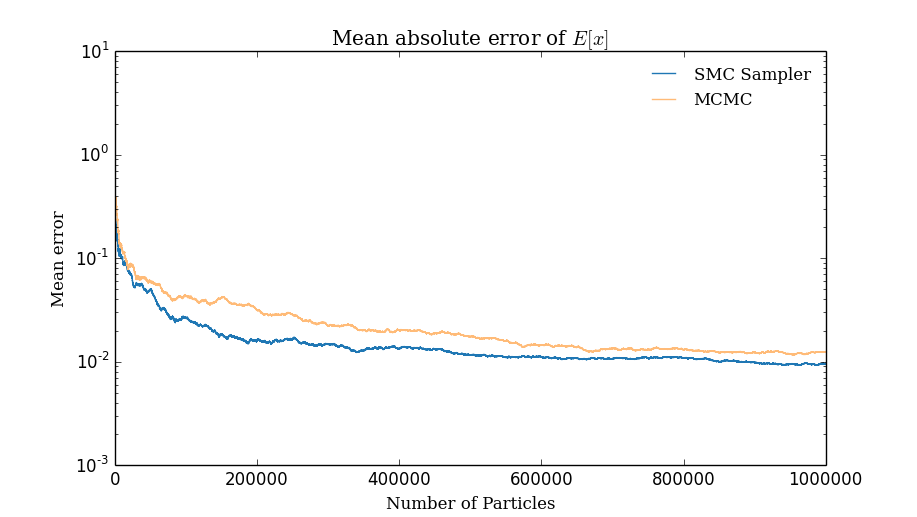
\includegraphics[width = \textwidth]{plots/E_X.png}
\caption{default}
\label{default}
\end{center}
\end{figure}

\begin{figure}[htbp]
\begin{center}
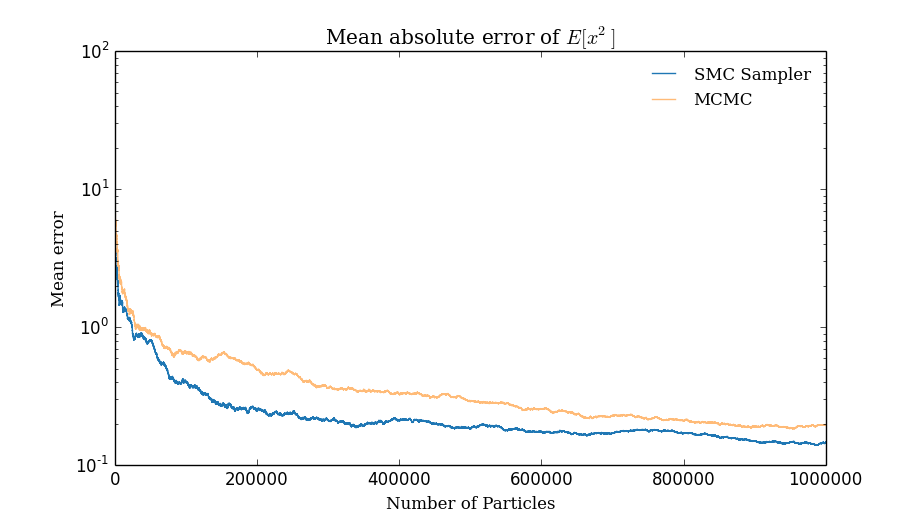
\includegraphics[width = \textwidth]{plots/E_X2.png}
\caption{default}
\label{default}
\end{center}
\end{figure}

\begin{figure}[htbp]
\begin{center}
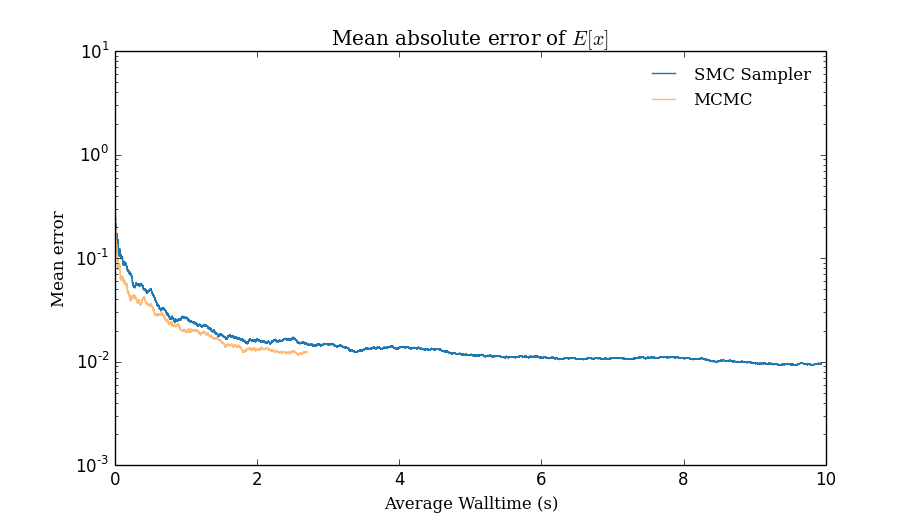
\includegraphics[width = \textwidth]{plots/E_X_walltime.png}
\caption{default}
\label{default}
\end{center}
\end{figure}

\begin{figure}[htbp]
\begin{center}
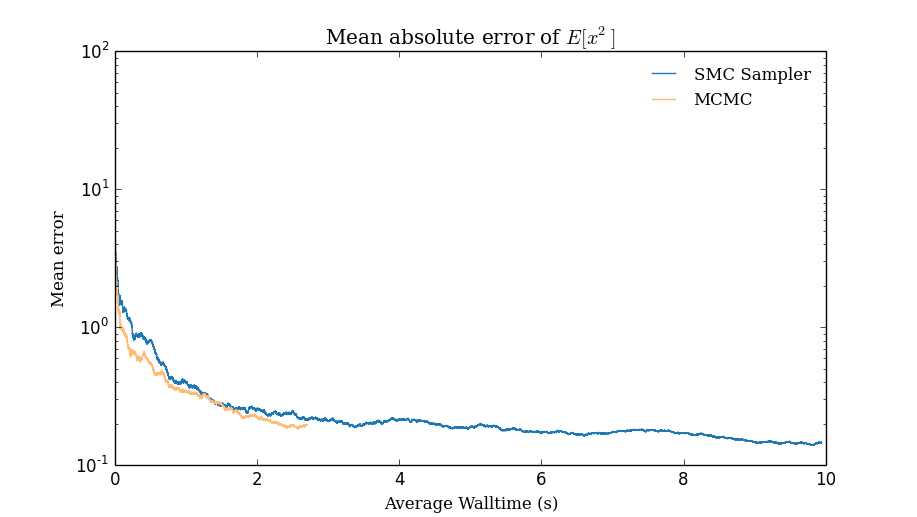
\includegraphics[width = \textwidth]{plots/E_X2_walltime.png}
\caption{default}
\label{default}
\end{center}
\end{figure}


\begin{figure}[htbp]
\begin{center}
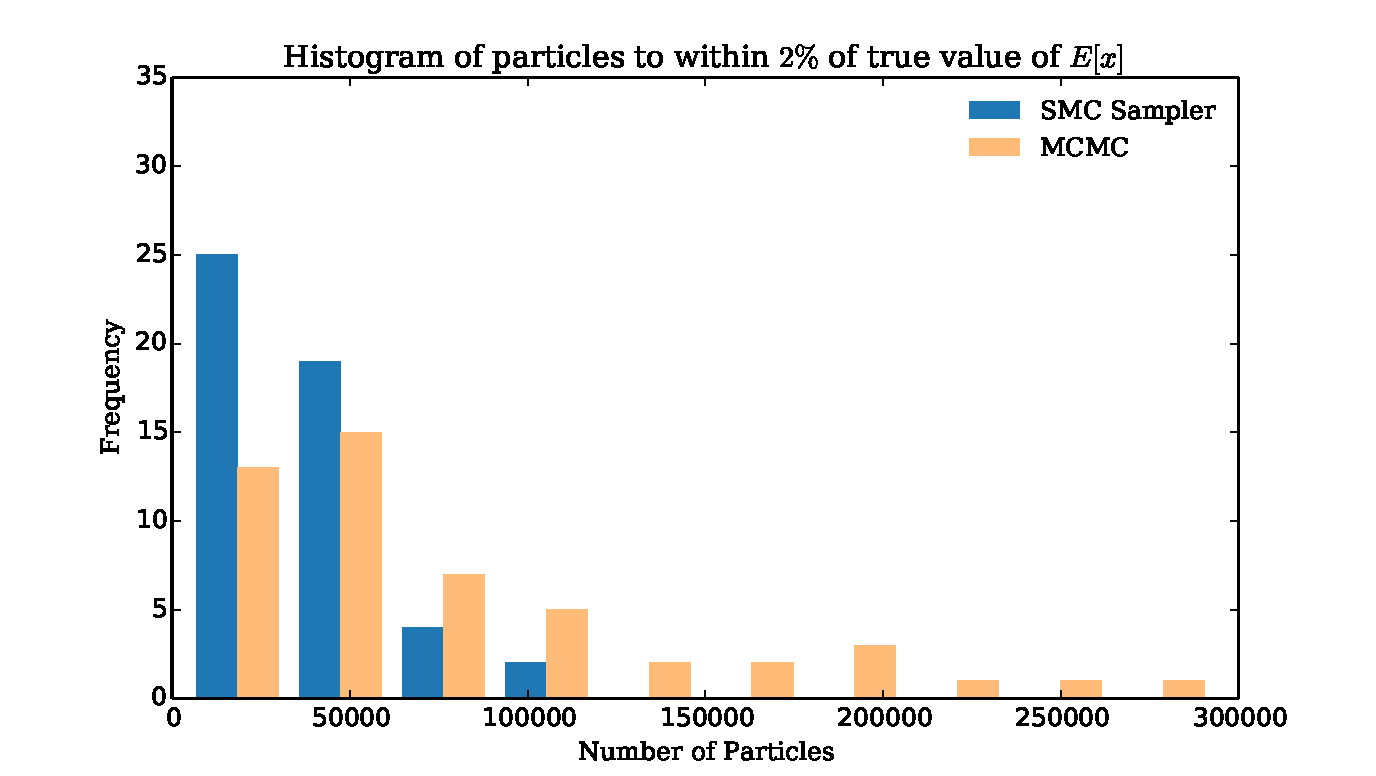
\includegraphics[width = \textwidth]{plots/iterations.pdf}
\caption{default}
\label{default}
\end{center}
\end{figure}

\begin{figure}[htbp]
\begin{center}
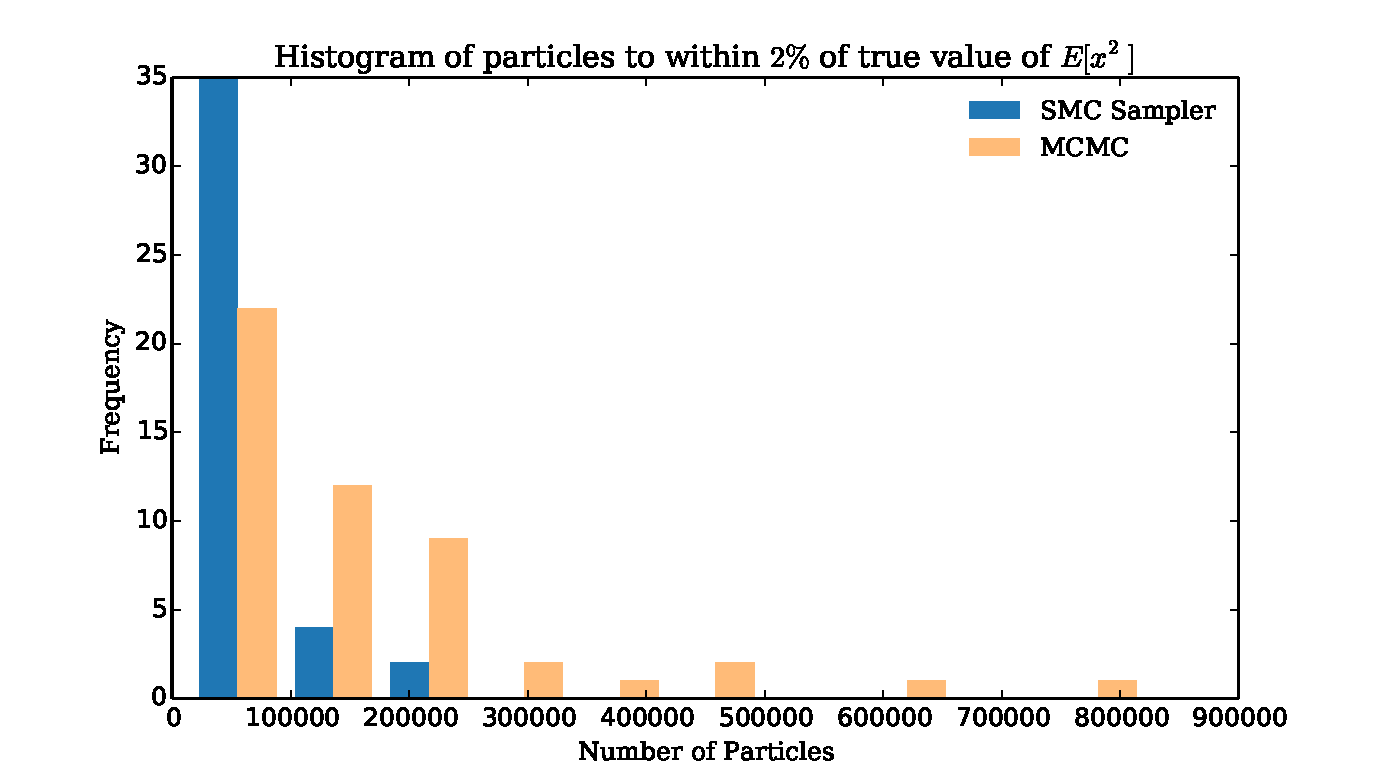
\includegraphics[width = \textwidth]{plots/iterationsEx2.pdf}
\caption{default}
\label{default}
\end{center}
\end{figure}



\bibliographystyle{model1-num-names}
\bibliography{sample.bib}

\end{document}